
\subsection{Presentation Layer}

\subsubsection{Introduktion}
Præsentationslaget i kasseapparatet er bygget med XML i WPF. Selve laget blev først designet ved brug af skitsen på figur \ref{fig:KasseMockup} og derefter implementeret med visual studios WPF designer som set på figur \ref{fig:EndeligeGUI}. Præsentationslaget er opsat i henhold til MVVM som sikrer at vores Præsentations- og Business Logic Lag er ordentligt adskilt.Til sidst til afsnittet er medtaget klassebeskrivelser der kort fortæller om hver klasse og dennes ansvar. \\

\subsubsection{Brugergrænsefladen}

\begin{figure}[H]
	\centering
	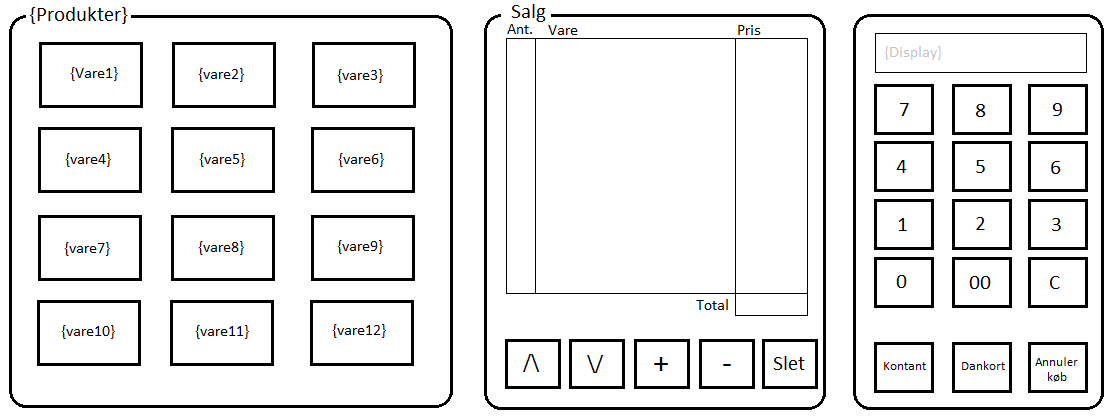
\includegraphics[width=1\textwidth]{Systemdesign/Frontend/pics/KasseMockup}
	\caption{Første mockup af grænsefladen til kasseapparatet.}
	\label{fig:KasseMockup}
\end{figure}

Den ovenstående skitse, var den første skitse af kasseapparatets brugergrænseflade som blev opsat. Denne skitse er tegnet i paint. Idéen bag grænsefladen var, at man skulle tænke fra højre mod venstre. Først vælges et produkt. Dette tilføjes til listen i midten. Når alle produkter er tilføjet færdiggøres salget i højre side af grænsefladen.

\begin{figure}[H]
	\centering
	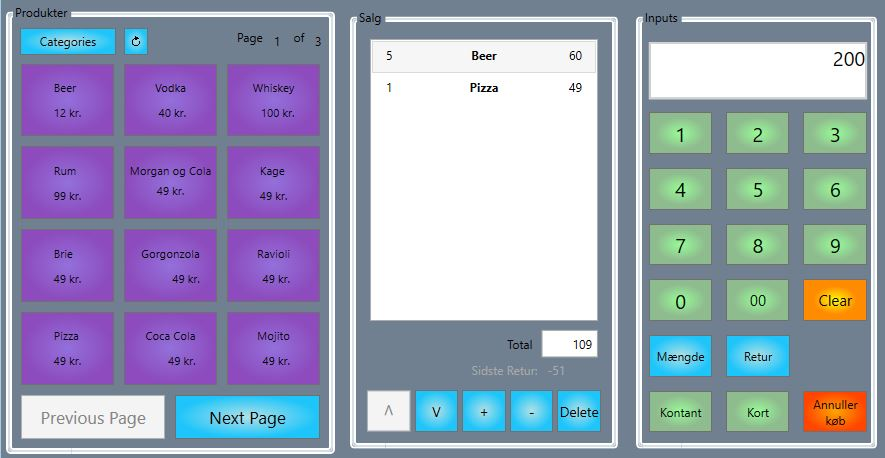
\includegraphics[width=1\textwidth]{Systemdesign/Frontend/pics/GUI}
	\caption{ProductButtonControl}
	\label{fig:EndeligeGUI}
\end{figure}

Som man kan se på de ovenstående figurer blev selve implementeringen af grænsefladen udført relativt tæt op af skitsen. Mere implementeringspecifikke deltaljer kommer herunder.

\newpage

\subsubsection{View}

Herunder vil de forskellige view filer kort blive beskrevet. \\

\subsubsection{Styling}

\textbf{ButtonStyle.xaml}

Da \gls{KA} \gls{GUI} indeholder mange knapper, er der lavet en stylings xaml fil for knapper, for at give \gls{KA} et mere karakteristisk udseende. Denne styling er også med til at dele de 3 segmenter i GUI'en mere op, og gøre det nemmer at benytte den hurtigere. \\
Styling filen består af RadialGradientBrushs, som giver knapperne et mere fysisk udseende. Stylingens filen er også tiltænkt at skulle give knapperne en afrundet border.

\begin{figure}[H]
	\centering
	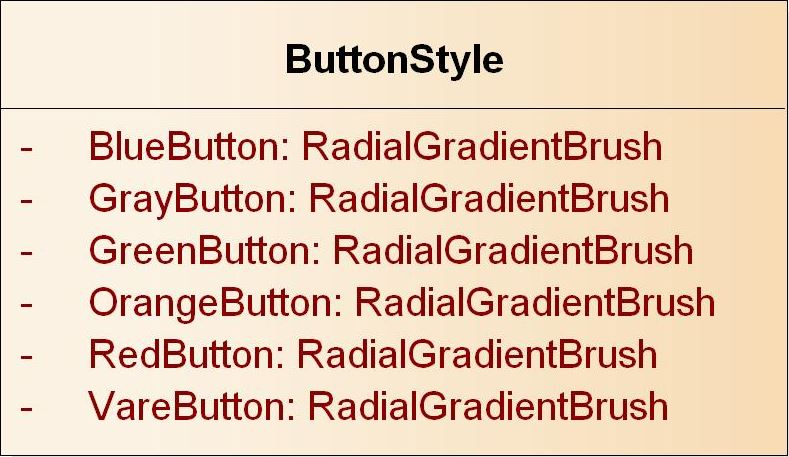
\includegraphics[width=60mm]{Systemdesign/Frontend/GUI/Pics/xaml}
	\caption{ButtonStyle.xaml}
	\label{fig:ButtonStyleXaml}
\end{figure}

\textbf{MainWindow.xaml}

Til kasseapparatet er der tilknyttet en stor Viewfil ved navn Mainwindow hvor hele opsætningen af grænsefladen visuelle dele er opskrevet. Hele grænsefladen er opbygget af grids. Ved at bruge grids er det nemt at opsætte grænsefladen, da man kan have grids i grids og derved præcist kan styre hvordan de forskellige elementer skal være placeret. Samtidig har grids indbygget skalering af de elementer den indkapsler. Dette gør at \gls{KS} selv skalerer korrekt alt efter skærmopløsningen.


\subsubsection{ViewModels}
Herunder vil de brugte viewmodels kort blivet forklaret.

\subsubsection{Klassebeskrivelser}
\textbf{MainWindow}\\
I MainWindow er der oprettet en række Button.Click.Events, som har ansvar for logic som er afhængig af displayet i inputs segmentet. Disse events er skrevet for at adskille ShoppingList fra selve view(xaml) delen og implementerer dermed en view(code) del, som laver funktionens kald ned til ShoppingList. 

\begin{figure}[H]
	\centering
	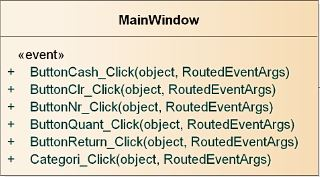
\includegraphics[width=80mm]{Systemdesign/Frontend/GUI/Pics/Main}
	\caption{MainWindow}
	\label{fig:KasseMainWindowClass}
\end{figure}

\textbf{CategoriesMenu}\\
CategoriesMenu er en menu med categorier. Denne klasse står for at kende alle kategorier. Ved et tryk på "Categories" knappen, vil CategoriesMenu oprette en menu med alle kategorier der eksisterer i systemet. Til hver MenuItem vil den også tilknytte en liste af produkter. Derved kan der, ved tryk på menuitem, oprettes knapper med præcis de produkter der er ønsket. 

\begin{figure}[H]
	\centering
	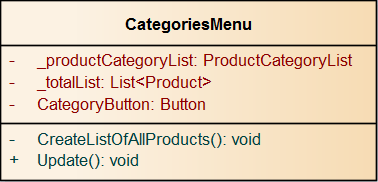
\includegraphics[width=0.3\textwidth]{Systemdesign/Frontend/pics/CategoriesMenu}
	\caption{CategoriesMenu.}
	\label{fig:PBC}
\end{figure}

\textbf{MenuCategory}\\
MenuCategory er en kategori i menuen. Den arver fra MenuItem som er et WPF element. Ved at oprette klassen på denne måde er det muligt at styre klassen direkte fra codebehind. Derved kan der tilknyttes commands, og det muliggør dynamisk oprettelse af MenuItems.


\begin{figure}[H]
	\centering
	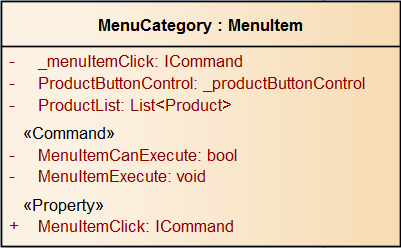
\includegraphics[width=0.3\textwidth]{Systemdesign/Frontend/pics/MenuCategory}
	\caption{MenuCategory.}
	\label{fig:PBC}
\end{figure}

\textbf{ProductButtonControl} \\
ProductButtonControl står for at styre hvilken knappeside der vises. Dette betyder at den indeholder en ProduktButtonList, der ved klik er i stand til at skifte knappeside.

\begin{figure}[H]
	\centering
	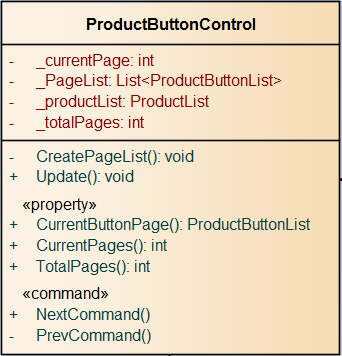
\includegraphics[width=0.3\textwidth]{Systemdesign/Frontend/pics/ProductButtonControl}
	\caption{ProductButtonControl.}
	\label{fig:PBC}
\end{figure}

\textbf{ProductButtonList} \\
ProductButtonList indeholder lister af knapper. Derved kan hver knappeliste symbolisere en side af knapper. Denne liste har ikke nogen anden funktionalitet, men eksisterer for at koden skal kunne facilitere dynamiske knappestørrelser i fremtiden. Denne klasse ville kunne tjekke på hvor stor siden er, og oprette knappesider med den ønskede antal knapper derefter.


\begin{figure}[H]
	\centering
	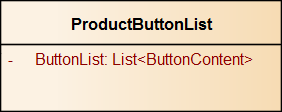
\includegraphics[width=0.3\textwidth]{Systemdesign/Frontend/pics/ProductButtonList}
	\caption{ProductButtonList.}
	\label{fig:PBL}
\end{figure}

\textbf{ProductButtonContent} \\
ProductButtonContent har indholdet af 1 knap på grænsefladen, samt produktinformationer og commands til at oprette produkter på ShoppingList ved tryk. Når man skifter side i grænsefladen vil ProductButtonContent være forbundet til hver knap.

\begin{figure}[H]
	\centering
	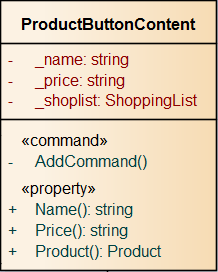
\includegraphics[width=0.2\textwidth]{Systemdesign/Frontend/pics/ProductButtonContent}
	\caption{ProductButtonContent.}
	\label{fig:PBCon}
\end{figure}
